\section{Alternative Models}



As seen above, once the dilution is large enough, we no longer detect the presence of Coho eDNA. Hence our statistical model should account for this asymptotic property. We fit and compare a variety of  non-linear models. These include the `broken stick' model for mean TCT, hyperbolic tangent models, Lowess models and finally a `Bent Cable Model' \citep{piecewiseregression}. In this analysis we include models fit to the response variable Mean Transformed CT. The models for median Transformed CT are very similar.

\subsection{Broken Stick Models}

Firstly, we fit what is known as a broken stick model. The broken stick model is a non-linear regression model that allows for sharp changes in direction.
The model includes a `break point', $\gamma$, that is used to fit a model. We use the R function `nls' \citep{nlsTools} which stands for `Nonlinear Least Squares' to fit the model. This function allows us to obtain `weighted' estimates of the parameters.

\vspace{3mm}

The Broken Stick model has the form:

\vspace{3mm}

 $$ \beta_{0}+\beta_{1}x+ \begin{cases}
0  &  \text{if    } x \le \gamma \\[2ex]
\beta_{2}(x-\gamma)  & \text{if    } x > \gamma
\end{cases}$$


This can be written as:

$$\beta_{0}+\beta_{1}x \hspace{1mm} \mbox{ for} \hspace{2mm} x \le \gamma \hspace{1mm} \mbox{, and}$$


$$\beta_{0}+\beta_{1}x+\beta_{2}(x-\gamma)=(\beta_{0}-\beta_{2}\gamma)+(\beta_{1}+\beta_{2})x \hspace{2mm} \mbox{for} \hspace{2mm}  x > \gamma \mbox{.} $$.


\begin{figure}[H]
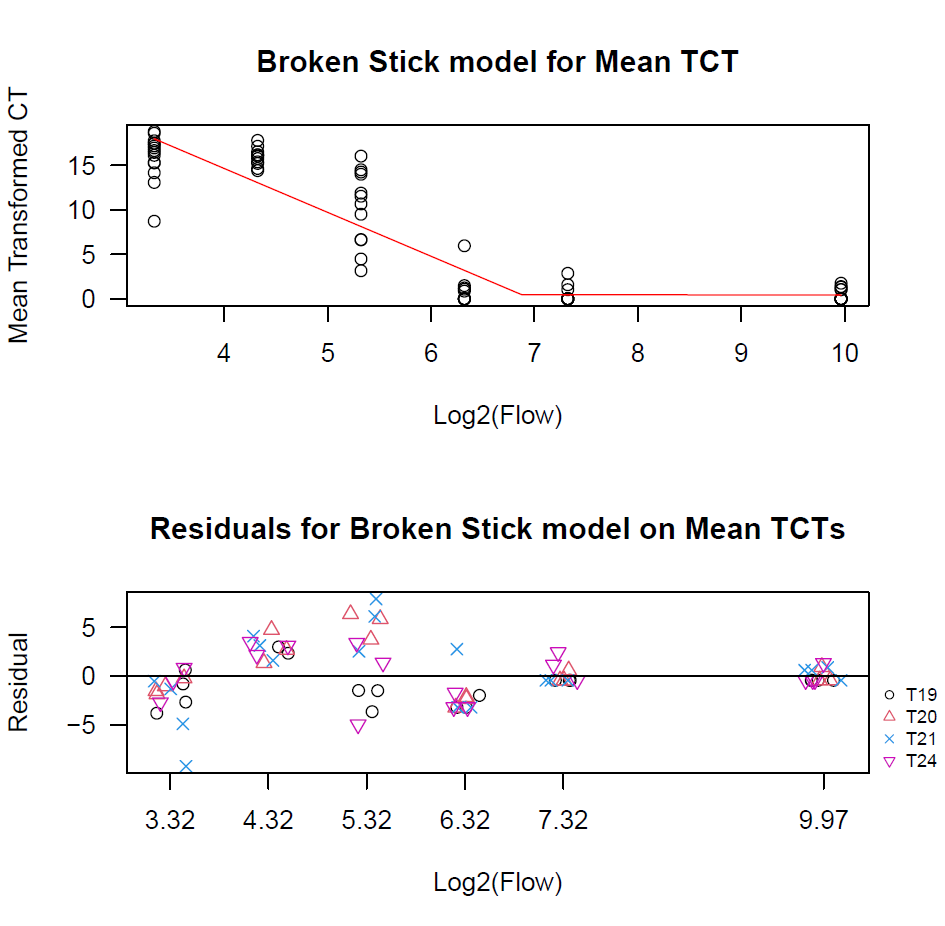
\includegraphics[scale=0.7]{Chapter4Images/meanbrokenstick.png}
\caption{Broken Stick model for Mean TCT (top) and the associated residuals for the model (bottom).}
\label{fig:brokenstickmean}
\end{figure}

%\begin{figure}[H]
%\includegraphics[scale=0.7]{tablesandimages/brokenstickmean1.pdf}
%\caption{Broken-Stick model for Mean Transformed CT and the associated residuals for the model }
%\label{fig:brokenstickmean}
%\end{figure}


Figure~\ref{fig:brokenstickmean} shows the broken stick regression line in red. The `breakpoint', $\gamma$ is estimate 6.877 (s.e 0.266). The estimate for $\beta_{0}$ is 33.374 (s.e 1.74), $\beta_{1}$ has an estimate of -4.931 (s.e 0.347) and $\beta_{2}$ is estimated to be 4.932 (s.e 0.555). Also included is the residual plot for the Broken-stick model. The fitted values are the predicted mean TCT for a given log2(Flow) value. On the y-axis are the actual residuals, the difference between the true value and the fitted value. The `RSS' (Residual Sum of Squares) for this model is 614.761.



\subsection{Bent Cable Models}


 In the previous analysis we fit broken stick models. We can see that in the broken stick models, the break point causes a sharp turn. However, it may be more reasonable and biologically sound to fit a more flexible model. Hence, we make use of the ``bent cable" model that allows for a smoother model \citep{bentcable}. We use the bentcable function \citep{bentcable2}.
 
 \vspace{5mm}
 
The Bent Cable model takes the form:
\vspace{5mm}


 $$ \beta_{0}+\beta_{1}x+ \begin{cases}
0  &  \text{if    } x < \alpha-\gamma \\[2ex]
\beta_{2}\frac{(x-\alpha+\gamma)^{2}}{4\gamma}  &  \text{if    } \alpha-\gamma  \le x \le \alpha+\gamma \\[2ex]
\beta_{2}(x-\alpha) & \text{if  } x > \alpha+\gamma
\end{cases}$$



\begin{figure}[H]
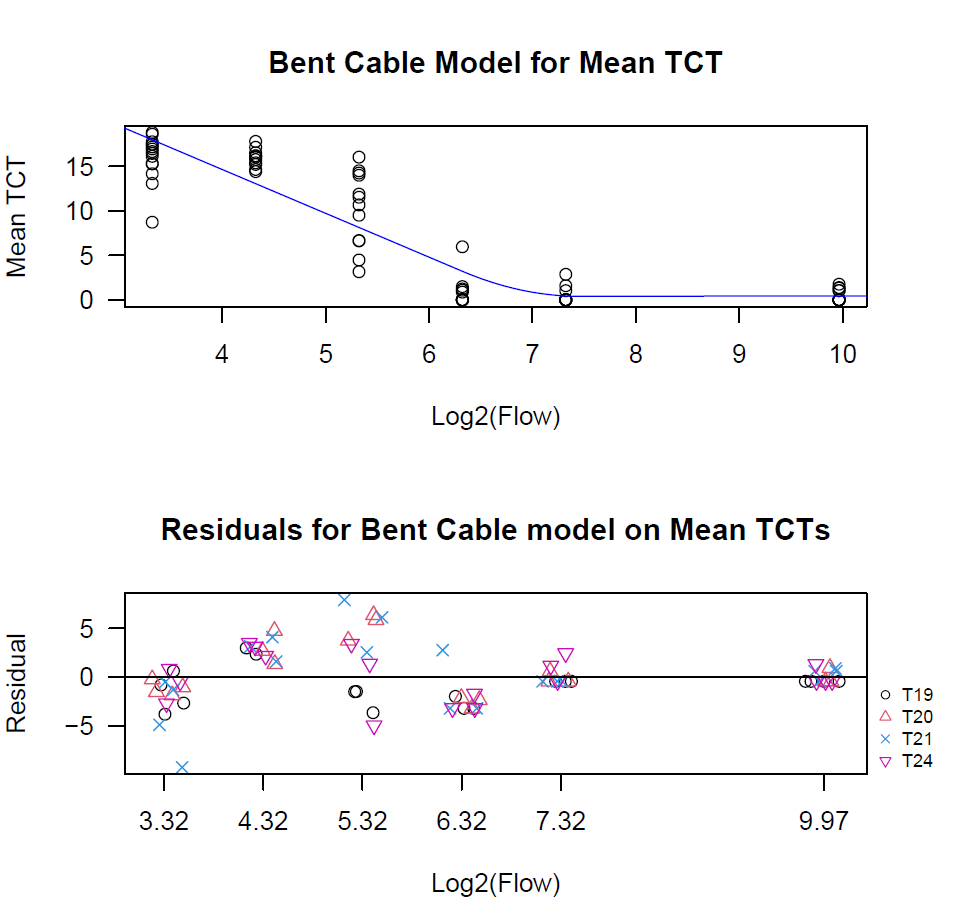
\includegraphics[scale=0.7]{Chapter4Images/meantctbentcable.png}
\caption{Bent Cable Model for Mean TCT (top) and the associated residuals for the model (bottom).}
\label{fig:meanbc}
\end{figure}





Figure~\ref{fig:meanbc}  is the plot of the bent cable model and the associated residual plot. The red line is the bent cable regression line. The $\alpha$ value is estimated as 6.89 (s.e 0.542), the $\gamma$ value is estimated 0.565 (s.e 0.124) and the log-likelihood  is -189.24. The estimate for $\beta_{0}$ is 34.350 (s.e 1.51), $\beta_{1}$ has an estimate of -4.925 (s.e 0.288) and $\beta_{2}$ is estimated to be 4.940 (s.e 0.550). The parameter $\alpha$ is the breakpoint discussed above, while $\gamma$ is a parameter that impacts the length of the quadratic portion connecting the two linear sections of the regression line. The RSS for this model is 614.767. 

\newpage

\subsection{Hyperbolic Tangent Models}

We can also fit models similar to `bent cables' that utilize the hyperbolic tangent function to allow for smoothness.

\vspace{12pt}
 
The tanh model takes the form:

$$\beta_{0}+\beta_{1}(x-\alpha)+\beta_{2}(x-\alpha)\tanh(\frac{x-\alpha}{\gamma})$$

where $\tanh(z)=\frac{e^{z}-e^{-z}}{e^{z}+e^{-z}}$ is the hyperbolic tangent function.



\begin{figure}[H]
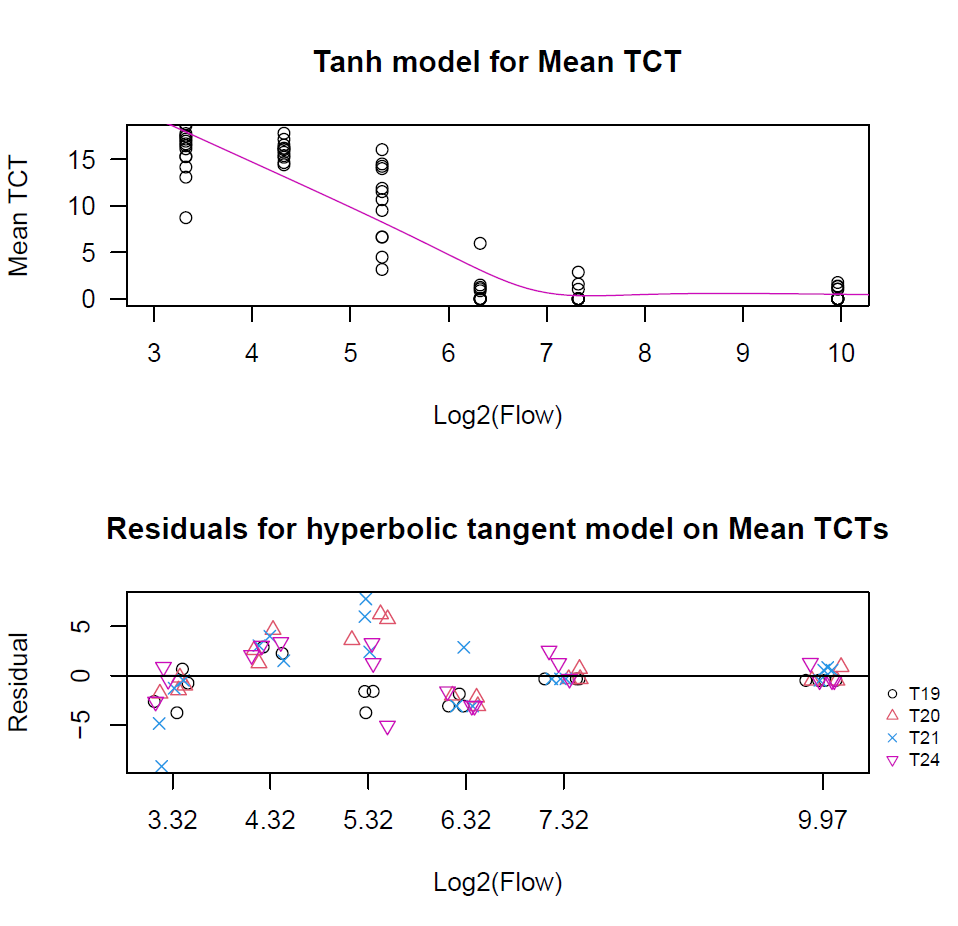
\includegraphics[scale=0.7]{Chapter4Images/tanhmodel.png}
\caption{Hyperbolic Tangent (tanh) model for Mean TCT (top) and the associated residuals for the model (bottom).}
\label{fig:meantanh}
\end{figure}


Figure ~\ref{fig:meantanh} is the tanh model and residuals for mean TCT. The purple line is the tanh regression line. For mean TCT, our hyperbolic tangent model estimates the break point `br' ($\alpha$) to be $\alpha=6.887$ (s.e 0.448). R estimates $\gamma= -0.776$ (s.e 4.82) , $\beta_{0}=0.8920$ (s.e 2.80), $\beta_{1}=-2.46$ (s.e 0.350) and $\beta_{2}=-2.33$ (s.e 1.03). The residuals look good as they appear to be randomly distributed about the y-axis. The RSS for the tanh model is 595.239.


\subsection{Lowess Models}

We fit similar models using the `lowess' function in R. lowess stands for locally-weighted polynomial regression.
 The lowess models are quite `sharp'. They both appear similar to our `broken stick' models. We used a smoothing parameter value of 3/4 and allowed the algorithm to perform three iterations.



\begin{figure}[H]
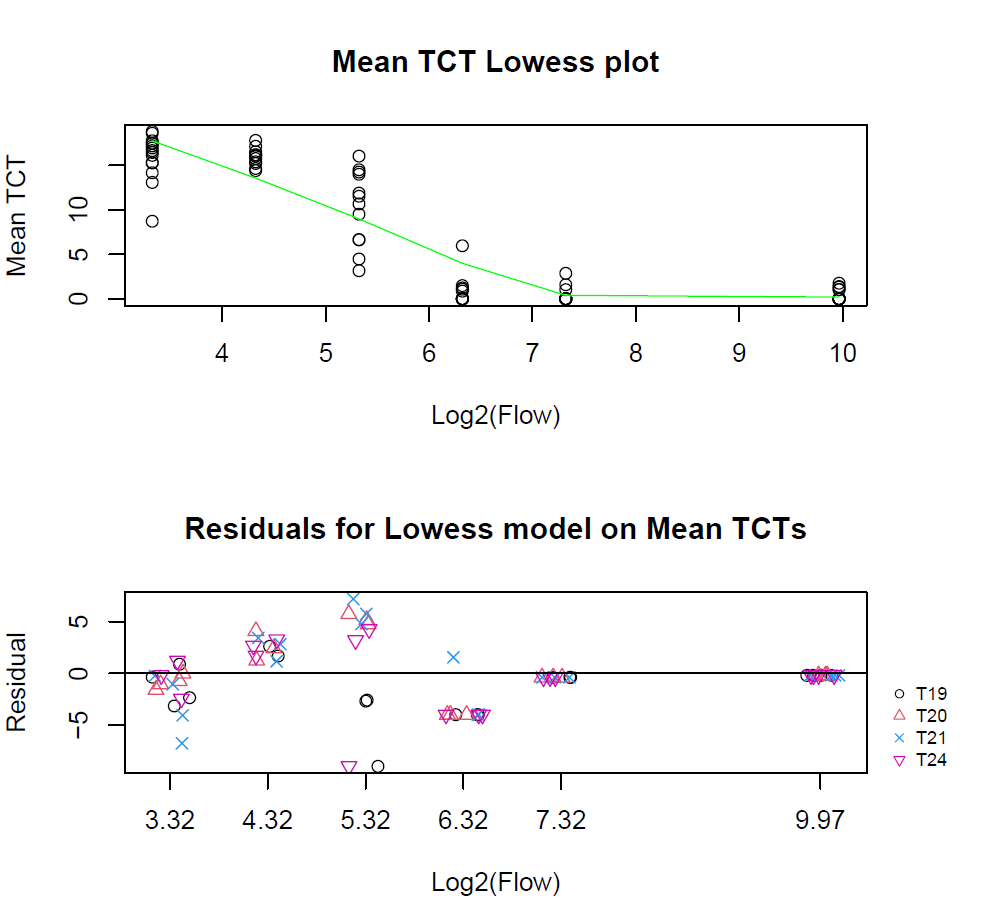
\includegraphics[scale=0.7]{Chapter4Images/meantctlowess.png}
\caption{Lowess model for Mean TCT (top) and the associated residuals for the model (bottom).}
\label{fig:meanlowess}
\end{figure}


Figure~\ref{fig:meanlowess} shows the lowess model for mean TCT and the associated residuals. The purple line represents the line of best fit according to the lowess criteria. This model looks very similar to the broken-stick model. This model estimates an intercept of 24.42 (s.e 0.894) and a lowess parameter of -2.74 (s.e 0.136). The residuals look good as they appear to be randomly distributed about the y-axis. The RSS for the lowess model is 589.698.




\newpage

\subsection{Model Comparison}

\begin{figure}[H]
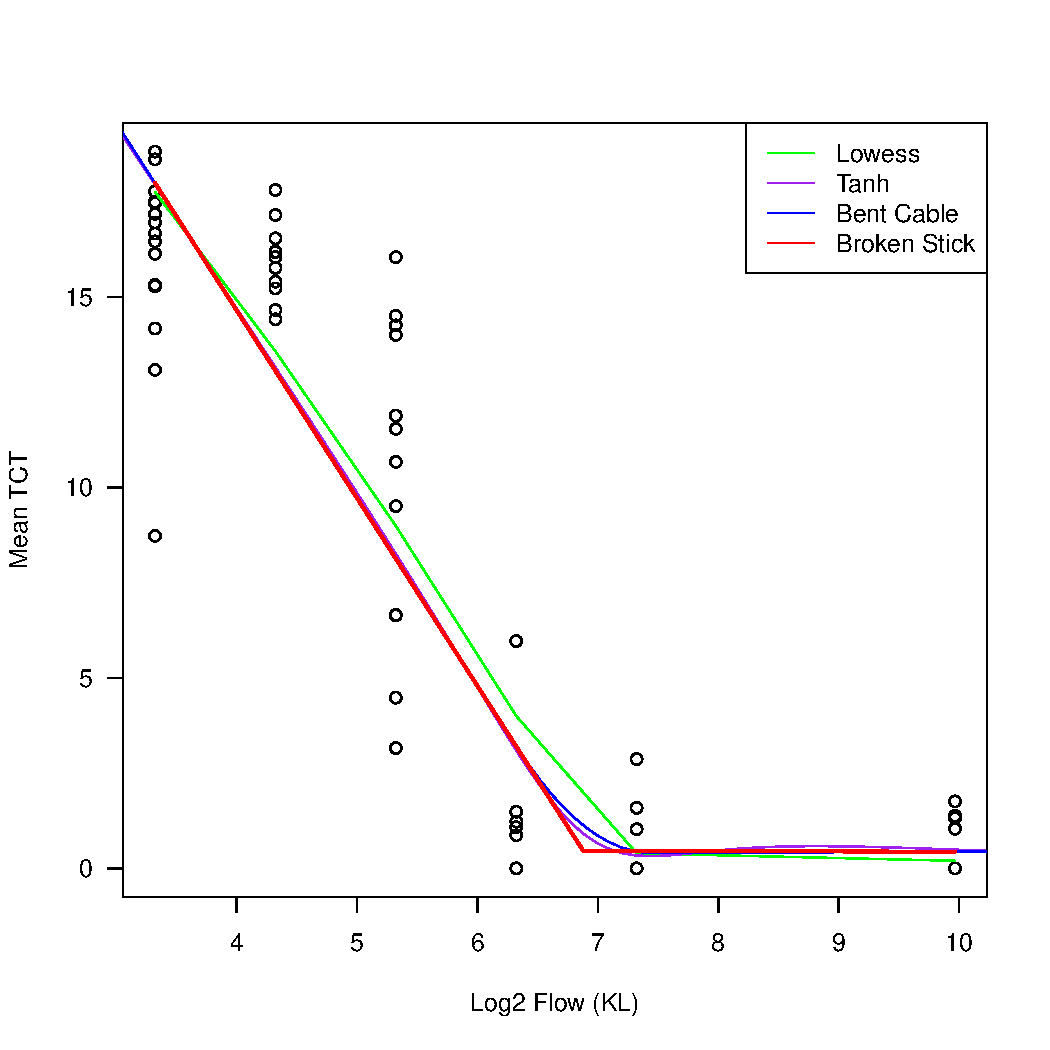
\includegraphics[scale=0.9]{Chapter4Images/meanTCTmodelcomparison.pdf}
\caption{Model comparison for four distinct models for the response variable mean TCT. Here we plot a broken-stick model, a lowess model, a hyperbolic tangent model and a bent-cable model.}
\label{fig:modelcomparison}
\end{figure}

Figure~\ref{fig:modelcomparison} plots all of our non-linear models for mean TCT. They all appear to be quite similar to one another. The broken-stick model appears to have a very sharp turn at the breakpoint, while the bent cable makes a more smooth transition.  The log-likelihood for the broken stick model is -189.24, which is the same as the log-likelihood for the bent-cable model. The log-likelihood for the Lowess and Tanh models is -185.34 and -187.99 respectively.


\begin{table}[H]
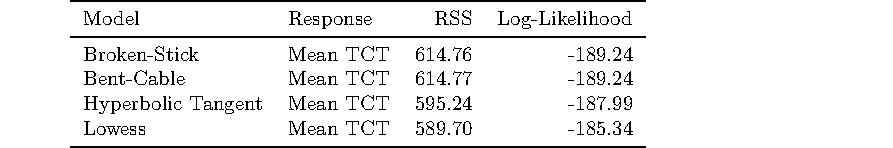
\includegraphics{Chapter4Images/nichealternate.pdf}
\caption{Model comparison for four distinct models for the response variable mean TCT. Here we plot a broken-stick model, a lowess model, a hyperbolic tangent model and a bent-cable model.}
\label{lab:comtable}
\end{table}


Table~\ref{lab:comtable} is a summary of our non-linear models. All four of the models are quite similar, and while the RSS for the bent-cable is slightly higher than that of the Lowess, we still chose to work with the Bent Cable due to the biological interpretation and smooth break point.


\newpage

The final model that we choose is the bent cable model. We choose this because it has a low log-likelihood and also makes biological sense. The bend represents the point of time in which eDNA is no longer detectable due to dilution. The RSS of the bent cable model is also not much larger than the RSS of the other three models.



\begin{figure}[H]
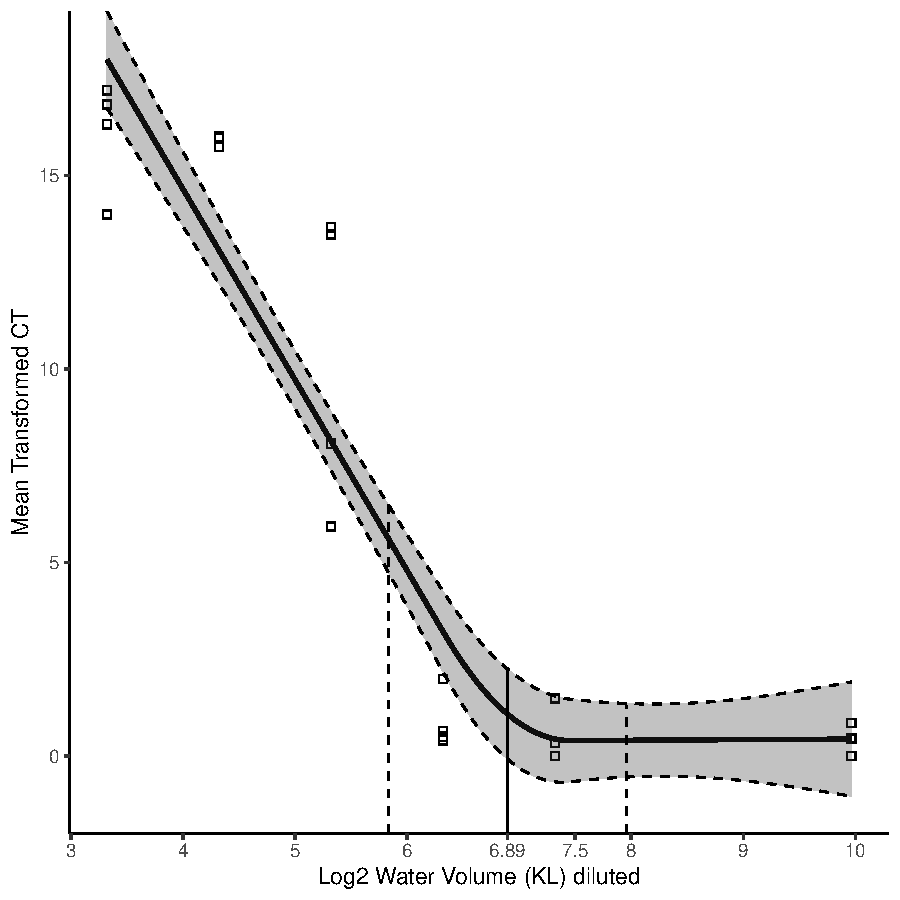
\includegraphics{Chapter4Images/flowggplot1.pdf}
\caption{ A bent cable model for mean TCT.}
\label{fig:bentcablemean}
\end{figure}


Figure~\ref{fig:bentcablemean} is a plot of our bent-cable model. The $\alpha$ value (estimated breakpoint) is 6.89 and is represented by the solid vertical line, the $\gamma$ value is 0.565 and the log-likelihood is -189.24. Included are the confidence regions for the regression line. Also included is the confidence interval for the breakpoint represented by the vertical dashed lines. The $\gamma$ value is a parameter that controls the length of the quadratic portion of the curve.